%!TEX root = 2024-cmsb_tool.tex
%Introduce what lumping is in the case of a rational system. 
Constrained lumping is a reduction method that allows to reduce a system in a way that it preserves a linear combination of variables of interest. 
Suppose we are interested in the evolution of an observable $x_1$ and its evolution is described by the following system of ODEs  
    \begin{equation} \label{eq:example1}
        \dot{x_{1}} = \frac {x_{2}^{2} +4x_{2}x_{3} +4x_{3}^{2}}{x_{1}^{2} + 1 },\qquad
        \dot{x_{2}} = \frac{2x_{1}-4x_{3}}{x_{2}+2x_{3} + 1},\qquad
        \dot{x_{3}} = \frac{-x_{1}-x_{2}}{x_{2}+2x_{3}+1}.
    \end{equation}
    The matrix $L = (1 \ 0\ 0, 0\ 1\  2)^{T}$ is an \textit{exact constrained lumping} of dimension 2, since it allows one to construct a smaller self-consistent system in terms of the \textit{macro-variables} $y_1= x_1$ and $ y_2 = x_2 + 2x_3$, as follows:
\begin{equation*}
        \begin{pmatrix}
            \dot{y}_{1} \\
            \dot{y}_{2}
        \end{pmatrix}
        =
        \begin{pmatrix}
            \dot{x}_{1} \\
            \dot{x}_{2} +2 \dot{x}_{3}
        \end{pmatrix}
        =
        \begin{pmatrix}
            \frac{(x_{2}+2x_{3})^{2}}{x_{1}^{2}+1} \\
            \frac{-2x_{2}-4x_{3}}{x_{2}+2x_{3}}
        \end{pmatrix}
        =
        \begin{pmatrix}
            \frac{y_{2}^{2}}{y_{1}^{2}+1} \\
            \frac{-2y_{2}}{y_{2}+1}
        \end{pmatrix}.
\end{equation*}
The matrix $L$ is a \textit{constrained} lumping since the evolution of $x_1$ can be directly recovered from the evolution of $y_1$.
It is \textit{exact} as there the evolution of $x_1$ can be recovered without any errors by using the lower dimensional system.
In general, given a system of ODEs $\dot{x} = f(x)$  and an exact lumping $L$ a self-consistent reduced system can be constructed as 
$y= L f(\bar{L}x)$, where $y = Lx$ and $\bar{L}$ is a right-pseudo inverse of $L$.

Now, suppose the evolution of $x_1$ is described by a slightly different system:
\begin{equation} \label{eq:examplepert}
	\dot{x}_{1} = \frac {x_{2}^{2} +4.05x_{2}x_{3} +4x_{3}^{2}}{x_{1}^{2} + 1 },~
	\dot{x}_{2} = \frac{2x_{1}-4x_{3}}{x_{2}+2x_{3} + 1},~
	\dot{x}_{3} = \frac{-x_{1}-x_{2}}{x_{2}+2x_{3}+1}.
\end{equation}
In this case, it is not possible to construct an exact approximate constrained lumping.
However, by relaxing the conditions for lumping the matrix $L = (1 \ 0\ 0, 0\ 1\  2)^{T}$ we can compute a smaller system that preserves $x_1$ up to an error, as follows.
\begin{equation*}
		\begin{pmatrix}
			\dot{y}_{1} \\
			\dot{y}_{2}
		\end{pmatrix}
		= L f \left(  \bar{L}        \begin{pmatrix}
			y_{1} \\
			y_{2}
		\end{pmatrix}
		\right)
		=
		L f \left(
		\begin{pmatrix}
				y_{1} & 0        \\
				0     & 0.2y_{2} \\
				0     & 0.4y_{2}
			\end{pmatrix} \right)
		=
		%L \begin{pmatrix}
		%1.004y_{2}^{2}    \\
		%2y_{1} - 1.6y_{2} \\
		%-y_{1}-0.2y_{2}
		%\end{pmatrix}=
		\begin{pmatrix}
			\frac{1.004y_{2}^{2}}{y_{1}^{2}+1} \\
			\frac{-2y_{2}}{y_{2}+1}
		\end{pmatrix}.
	\end{equation*}
\begin{wrapfigure}[12]{r}{0.4\textwidth}
		\centering
        \vspace{-0.5cm}
		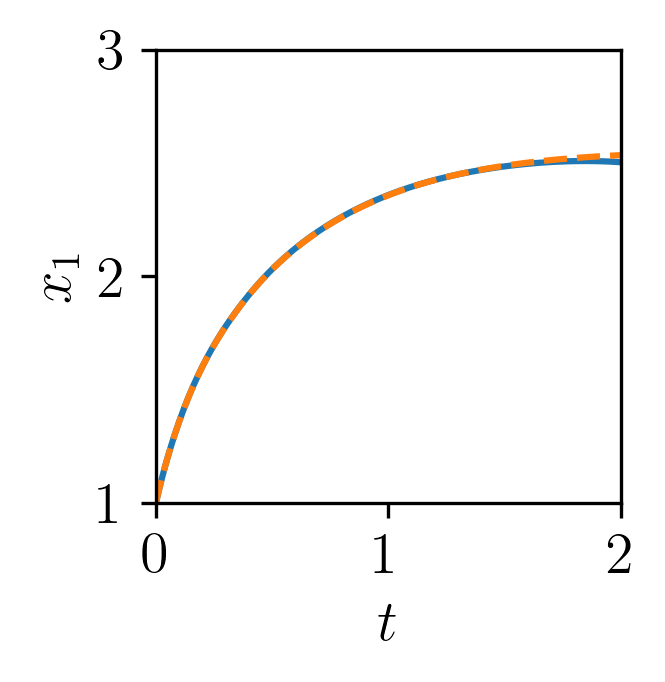
\includegraphics[width=0.7\linewidth]{./img/sim_red_example.png}
		\caption{Evolution of the reduced (orange) and original (blue).}
		\label{fig:apperr:sim}
\end{wrapfigure}
This means that the evolution of $x_1$ will be recovered up to an error.
Figure~\ref{fig:apperr:sim} shows the evolution of $x_1$ computed via the original and reduced system for initial conditions $x = (1,0,0)^{T}$
Note that by using an approximate reduction it is possible to reduce a system that was not exactly reducible while still obtaining a simulation with low error.
The detailed theory or approximate constrained lumping for polynomial systems, including the algorithm to compute them and how to bound the introduce errors, can be found in~\cite{leguizamon-robayo_approximate_2023}.



%In general, for an ODE system $\dot{x}= f(x)$  
%Consider a system of ODEs $\dot{x}= f(x)$, where $f: \mathbb{R}^{n}\to \mathbb{R}^{n}$ and each entry of $f$ is a rational function. 
%We say that a linear transformation $L: \mathbb{R}^{n}\to \mathbb{R}^{m}$ with $m< n$ is an \textit{exact lumping} if there exists a function $g:\mathbb{R}^{m} \to \mathbb{R}^{m}$, such that $L\circ f = g \circ L$. 
%For an initial condition $x(0) \in \mathbb{R}^n$ and an exact lumping $L$, there is a corresponding initial condition $y(0)$ in the lumped variables given by $y(0) = L x(0)$.
%A self-consistent system of ODEs can be constructed as follows \[L\dot{x} = Lf(x)= g(Lx)=g(y)=\dot{y}\ .\]



%Assume now that the dynamics are given by 
%\begin{equation} \label{eq:examplepert}
	%\dot{x}_{1} = \frac {x_{2}^{2} +4.05x_{2}x_{3} +4x_{3}^{2}}{x_{1}^{2} + 1 },~
	%\dot{x}_{2} = \frac{2x_{1}-4x_{3}}{x_{2}+2x_{3} + 1},~
	%\dot{x}_{3} = \frac{-x_{1}-x_{2}}{x_{2}+2x_{3}+1}.
%\end{equation}
%We still want to preserve the observable $x_1$. 
%In this case, the matrix $L = (1 \ 0\ 0, 0\ 1\  2)^{T}$ is not 



%In this paper, we study systems of ODEs with analytic derivatives of the form:
%\begin{equation}
	%\dot{x}  = f(x), \label{eq:ode}
%\end{equation}
%where $f: \mathbb{R}^{m} \to \mathbb{R}^{m}, x\mapsto (f_{1}(x), \dots, f_{m}(x))^{T}$ and $f_{i}$ is an analytic function,  for $i=1,\dots, m$.

%\begin{definition}\label{def:lump}
	%Given a system of ODEs of the form given by Equation~\eqref{eq:ode}, and a full rank matrix $L\in \mathbb{R}^{l\times m}$ with $l< m$,
	%we say that $L$ is an \emph{exact lumping of dimension $l$} (or that the system is \emph{exactly lumpable} by $L$) if there exists a function $g: \mathbb{R}^{l} \to \mathbb{R}^{l}$ with polynomial entries such that $Lf = g\circ L$.
%\end{definition}


%\begin{definition}\label{def:constlump}
	%Given a system of ODEs of the form given by Equation~\eqref{eq:ode}, and an exact lumping $L\in \mathbb{R}^{l\times m}$, we say that $y= Lx$ are the \emph{reduced (or lumped) variables}, 	and their evolution is given by the \emph{reduced system} $ \dot{y}= g(y)$.
%\end{definition}

%Given an initial condition $x^{0} \in \mathbb{R}^n$ and an exact lumping $L$, there is a corresponding initial condition $y^{0}$ in the lumped variables given by $y^{0} = L x^{0}$.
%Similarly, since $y=Lx$ and $g\circ L = Lf$, we have that \[L\dot{x} = Lf(x)= g(Lx)=g(y)=\dot{y}\ .\]
%This means that we can study the evolution of the lumped variables $y(t)$ by solving the (smaller) reduced system rather than the (larger) original one.

%Suppose that we want now to recover the evolution of some linear combination of state variables.
%To answer whether this is possible, we introduce the notion of constrained lumping.

%\begin{definition}
	%Let $x_{obs}= Mx$ for some matrix $M \in \mathbb{R}^{p\times m}$, for $p< m$.
	%We say that a lumping $L$  is a \emph{constrained lumping} with \emph{observables} $x_{obs}$ if  $\rsp(M) \subseteq \rsp(L)$.
	%This means that each entry of $x_{obs}$ is a linear combination of the reduced 	variables $y$. 	
%\end{definition}

%\begin{myExample}
	%Suppose we are interested in observing the quantity $2x_{1}+x_{2}+2x_{3}$ where the evolution is given by the system~\eqref{eq:example1}.
	%In this case $x_{obs}= Mx$ with $M = ( 2\ 1\ 2)$.
	%We can see that  $L$ from Example \ref{ex:firstode} is a constrained lumping as we can recover the observable from the reduced system, i.e., $ x_{obs}=2y_{1}+y_{2}$.
	%Suppose now that we want to observe the quantity $x_{1}+x_{2}+x_{3}$.
	%In this case $M = ( 1\ 1\ 1)$ and so the matrix $L$ is not a constrained lumping as there is no way to obtain $x_{obs}$ as a linear combination of $y_{1}$ and $y_{2}$.
%\end{myExample}

%To understand how a constrained lumping can be computed, we first review the following known characterization of lumping.

%\begin{theorem}[Characterization of Exact Lumping~\cite{tomlin_effect_1997}]\label{thm:lumping}
	%Given a system of $m$ ODEs of the form given by Equation\eqref{eq:ode} and a matrix $L\in \mathbb{R}^{l\times m}$ with rank $l$, the following are equivalent.
	%\begin{enumerate}
		%\item The system is exactly lumpable by $L$.
			  %\item\label{thm:lumping:inverse} For any pseudoinverse $\bar{L}$ of $L$, $Lf = (Lf) \circ \bar{L}L$.
			  %\item\label{thm:lumping:invariant} The row space of $L$ is invariant under $J(x)$ for all $x\in \mathbb{R}^{m}$, where $J(x)$ is the total derivative of $f$ at $x$, known also as the Jacobian.
			  %More formally, $\rsp(L J(x)) \subseteq \rsp(L)$ for all $x \in \RE^m$.
	%\end{enumerate}
%\end{theorem}

%The characterization of exact lumpings in Theorem~\ref{thm:lumping} provides us a way to compute a constrained lumping $L$.
%This is because thanks to Point~\ref{thm:lumping:invariant}, the problem of computing a lumping is equivalent to the problem of finding a $J(x)$-invariant subspace of $\mathbb{R}^{m}$ for all $x \in \mathbb{R}^{m}$.
%However, $J(x)$ is a matrix whose entries are functions of $x$.
%In other words, there is a different real-valued matrix for each $x \in \mathbb{R}^{m}$.
%To circumvent this issue we require the following result:

%\begin{theorem}[{\cite[Lemma 1]{jimenez_clue_2022}}]\label{thm:repJ}
	%Consider a system ODEs of the form given by Equation~\eqref{eq:ode} and let $J(x)$ be the Jacobian matrix of $f$.
	%Let $\mathcal{B}$ be any set of real-valued matrices spanning the $\mathbb{R}-$vector space $$\mathcal{V}_{J}:=\left< J(x) | x \in \mathbb{R}^{m} \text{ and $J(x)$ is well-defined}\right>.$$
	%Then $L$ is a lumping of~\eqref{eq:ode} if and only if $\rsp(L)$ is invariant to each $J_i \in \mathcal{B}$.
%\end{theorem}

%A set of matrices $\{J_1,\dots, J_N\}$ can be found analytically when $J(x)$ can be represented as
%\begin{equation}\label{eq:jacrep}
	%J(x) = \sum_{i=0}^{N}J_{i}\mu_{i}(x),
%\end{equation}
%where $\left\{\mu_{i}(x)\ :\ i\in\{0,\ldots,N\}\right\}$ is a set of analytic functions.
%When working with polynomial systems, each of the entries of $J(x)$ is a polynomial and so each $\mu_i$ corresponds to the monomials of $J(x)$.

%\comalex{
	%In particular, for rational systems, a  similar representation of $J(x)$ can be obtained symbolically by differentiating $f(x)$ and then multiplying by the minimum common denominator.
	%In practice, this approach is computationally unfeasible due to the fact that this symbolic approach results in an explosion of the number of monomials in $J(x)$.
	%\coma{sentence difficult to parse. Does it explode after differentiating (i.e. we differentiate after using the mcd? or we apply the mcd after differentiating?}
	%To avoid any explicit symbolic computations, a representation $\{J_1,\dots, J_N\}$ can be obtained by sampling $f(x)$ at different points and using automatic differentiation.
	%%In this way, we avoid any explicit symbolic computation of the Jacobian matrix.
	%The general idea of this sampling procedure is formalized by Algorithm~\ref{alg:findJ}.
	%Our implementation followed the recommendations found in~\cite[Section 3.4]{jimenez_clue_2022}.
	%These guidelines show how to efficiently sample $J(x)$ to obtain a correct representation of $\mathcal{V}_{J}$ with high probability.

	%\begin{algorithm}[h]
		%\caption{\footnotesize Representing $J(x)$}\label{alg:findJ}
		%%\algsetup{linenosize=\tiny}
		%%\scriptsize
		%\begin{algorithmic}[1]
			%\REQUIRE
			%$f: \mathbb{R}^{m} \to \mathbb{R}^{m}$\\
			%a compact set $\Omega \subset \mathbb{R}^{m}$\\
			%\STATE {\textbf{set} $N=0$}
			%\REPEAT
			%\STATE {\textbf{set} $N=N+1$}
			%\STATE {\textbf{compute} $x_N$ sampling uniformly from $\Omega$ }
			%\STATE {\textbf{compute} $J_N=J(x_N)$ using automatic differentiation}
			%\UNTIL{$J_N \in \left< J_i | 1\leq i \leq N-1 \right>$}

			%\RETURN {$\{J_1,\dots, J_{N-1}\}$}.
		%\end{algorithmic}
	%\end{algorithm}

	%\coma{Before talking about alg 1 we need to introduce it. We shall say: This can be implemented as shown in Algorithm~\ref{alg:findJ}, using the recommendations... }
	%%The following example shows Algorithm~\ref{alg:findJ} in action.

	%\comalex{
		%\begin{myExample}\label{ex:findJ}
			%Consider the system given by  Example~\ref{ex:firstode}.
			%In this case, we first use the analytic approach to find a basis for $\mathcal{V}_{J}$.
			%By symbolically differentiating and multiplying by the minimum common denominator, we infer that the Jacobian of $f(x)$ is of the form $J(x)= B(x)/q(x)$ where the minimum common denominator is
			%$ q(x)= (x_{1}^{2} +1)^{2}(x_{2}+2x_{3}+1)^{2}$
			%and $B(x)$ is a matrix with polynomial entries up to degree 5.
			%Notice that to obtain a representation we need to expand all the terms in $B(x)$.
			%%[(5, (1, 5, 2)), (5, (3, 3, 2)), (5, (5, 2, 3)), (5, (2, 4, 3))]
			%These symbolic computations can be avoided by using Algorithm~\ref{alg:findJ}.
			%Following~\cite{jimenez_clue_2022}, we find that the dimension of $\mathcal{V}_{J}$ is 6.
			%The set $\{J_1,\dots,J_6\}$ is obtained by evaluating $J(x)$ at the following points: $
				%x_1 = (1, 5, 2),~x_2 = (3, 3, 2),~x_3 = (5, 2, 3),~x_4 = (2, 4, 3),~x_5 = (3, 2, 4),~x_6 = (4, 3, 2).$
			%For the sake of brevity, we only display the first 4 matrices $J_i$:
			%%[ 0  0  0  2 -2 -8 -1  0  2]
			%%[ 0.    2.    4.    1.    0.   -2.   -0.5  -0.25  0.5 ]
			%%[ 0.     4.     8.     0.667  0.444 -0.444 -0.333 -0.333  0.   ]
			%%[-40.5    9.    18.     0.2    0.06  -0.28  -0.1   -0.04   0.12]
			%\begin{equation*}
				%\begin{split}
					%J_1 &=
					%\begin{pmatrix}
						%0  & 0  & 0  \\
						%2  & -2 & -8 \\
						%-1 & 0  & 2
					%\end{pmatrix},\\
					%J_3 &=
					%\begin{pmatrix}
						%0      & 4      & 8      \\
						%0.667  & 0.444  & -0.444 \\
						%-0.333 & -0.333 & 0
					%\end{pmatrix},
				%\end{split}
				%\hspace{1cm}
				%\begin{split}
					%J_2 &=
					%\begin{pmatrix}
						%0    & 2     & 4   \\
						%1    & 0     & -2  \\
						%-0.5 & -0.25 & 0.5
					%\end{pmatrix},\\
					%J_4 &=
					%\begin{pmatrix}
						%-40.5  & 9      & 18     \\
						%0.200  & 0.060  & -0.280 \\
						%-0.100 & -0.040 & 0.120
					%\end{pmatrix}.
				%\end{split}
			%\end{equation*}
		%\end{myExample}
	%}
	%%\coma{The alignment is completely messed up. Can we at least align the '='?}


	%We see that Algorithm~\ref{alg:findJ} outputs a set of matrices $\{ J_1,\dots, J_N\}$
	%%\coma{$N$ or $M$? the algorithm says $M$} 
	%spanning $\mathcal{V}_{J}$.
	%Given such a set, Theorem~\ref{thm:repJ} provides an algorithmic way to find a constrained lumping $L$ by performing a finite number of checks over real-valued vectors.
	%This is shown in Algorithm~\ref{alg:findL}.
	%The use of Algorithms~\ref{alg:findJ} and~\ref{alg:findL} to obtain a constrained lumping $L$ is summarized in Algorithm~\ref{alg:clue}.
	%%The aforementioned reasoning gives rise to a computational way to verify Point~\ref{thm:lumping:invariant} in Theorem~\ref{thm:lumping}, i.e.,  Algorithm~\ref{alg:clue}.
	%\coma{It is a bit weird that we cite Alg3 before Alg2. Can we rephrase this sentence?}
	%%Using Equation~\eqref{eq:jacrep},the condition of Theorem~\ref{thm:repJ} can by checked by noticing that all rows $r$ of $L$, $rJ(x) \in \rsp(L)$ for all $x$ if and only if $rJ_{i} \in \rsp(L)$ for $i=1,\dots, N$.
	%%This result leads to Algorithm~\ref{alg:findL}.

	%\hspace{-0.65cm}
	%\begin{minipage}[t]{0.47\textwidth}
		%\begin{algorithm}[H]
			%\caption{\footnotesize Computation of $L$}\label{alg:findL}
			%\algsetup{linenosize=\tiny}
			%\scriptsize
			%\begin{algorithmic}[1]
				%\REQUIRE
				%a set of matrices $\left\{ J_1,\dots,J_N \right\}$ spanning $\mathcal{V}_{J}$ (Theorem \ref{thm:repJ});\\
				%a $p \times m$ matrix $M$ with row rank $p$.\label{alg:findL:M}

				%\STATE \textbf{set} $L := M$
				%\REPEAT
				%\FORALL{$1 \leq i \leq \kappa$ and rows $r$ of $L$}
				%\STATE {\textbf{compute} $r J_i$ }
				%\IF{$rJ_{i}\notin \rsp(L)$} \label{alg:findL:check}
				%\STATE {\textbf{append} row $r J_i$ to $L$}\label{alg:findL:append}
				%\ENDIF
				%\ENDFOR
				%\UNTIL{no rows are appended to $L$}

				%\RETURN Lumping matrix $L$.
			%\end{algorithmic}
		%\end{algorithm}
		%\vspace{0.01cm}
	%\end{minipage}
	%\hfill
	%\begin{minipage}[t]{0.47\textwidth}
		%\begin{algorithm}[H]
			%\caption{\footnotesize Constrained lumping \cite{ovchinnikov_clue_2021} }\label{alg:clue}
			%\algsetup{linenosize=\tiny}
			%\scriptsize
			%\begin{algorithmic}[1]
				%\REQUIRE \!\!a\! system \!$\dot{x} \!=\!\! f(x)\!$ of $\!m\!$ \! ODEs;\\
				%a $p \times m$ matrix $M$ with row rank $p$.\\

				%%\STATE \textbf{compute} $J(x)$, the Jacobian 			of $f(x)$

				%\STATE \textbf{compute} a set of matrices $\left\{ J_1,\dots,J_N \right\}$ spanning $\mathcal{V}_{J}$ (Algorithm~\ref{alg:findJ})\\
				%\STATE \textbf{compute} $L$ (Algorithm \ref{alg:findL}) \label{alg:clue:findL}

				%\RETURN Constrained lumped ODE system $\dot{y} = L f (\bar{L}y)$.

			%\end{algorithmic}
		%\end{algorithm}
		%\vspace{0.01cm}
	%\end{minipage}


	%The number of checks in Algorithm~\ref{alg:findL} is proportional to the number of elements in $\mathcal{V}_{J}$.
	%Moreover, Algorithm~\ref{alg:findL} can be implemented with polynomial time complexity~\cite{ovchinnikov_clue_2021,jimenez_clue_2022}.
	%%\coma{problems with English. do we mean have polynomial time complexity?}

%}

